\begin{table}[!hbt]
	\centering
    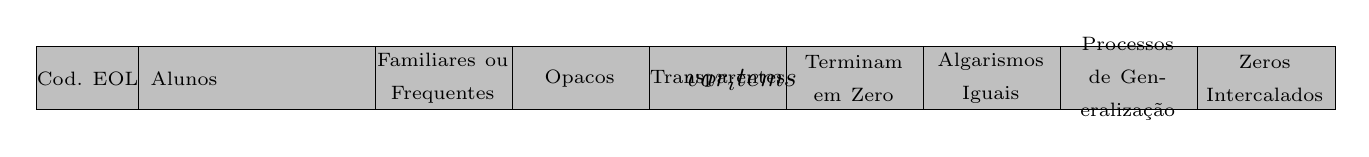
\begin{tikzpicture} 
		\fill[lightgray] (-8.25,0.5) rectangle (8.25,-0.3);
        \draw (-8.25,0.5) rectangle (8.25,-0.3);
        
        \draw (-6.95,0.5) -- (-6.95,-0.3);
        \draw (-3.94,0.5) -- (-3.94,-0.3);
        \draw (-2.2,0.5) -- (-2.2,-0.3);
        \draw (-0.46,0.5) -- (-0.46,-0.3);
        \draw (1.28,0.5) -- (1.28,-0.3);
        \draw (3.02,0.5) -- (3.02,-0.3);
        \draw (4.76,0.5) -- (4.76,-0.3);
        \draw (6.5,0.5) -- (6.5,-0.3);

        \node at (-7.60,0.1) {\fontsize{7}{0}\selectfont Cod. EOL};
        \node[text width=2.9cm] at (-5.35,0.1) {\fontsize{7}{0}\selectfont Alunos};
        \node[text width=1.7cm, align=center] at (-3.09,0.1) {\fontsize{7}{0}\selectfont Familiares ou Frequentes};
        \node[text width=1.7cm, align=center] at (-1.35,0.1) {\fontsize{7}{0}\selectfont Opacos};
        \node[text width=1.7cm, align=center] at (0.39,0.1) {\fontsize{7}{0}\selectfont Transparentes};
        \node[text width=1.7cm, align=center] at (2.13,0.1) {\fontsize{7}{0}\selectfont Terminam em Zero};
        \node[text width=1.7cm, align=center] at (3.87,0.1) {\fontsize{7}{0}\selectfont Algarismos Iguais};
        \node[text width=1.7cm, align=center] at (5.61,0.1) {\fontsize{7}{0}\selectfont Processos de Generalização};
        \node[text width=1.7cm, align=center] at (7.35,0.1) {\fontsize{7}{0}\selectfont Zeros Intercalados};


$var_items$
        

	\end{tikzpicture}
\end{table}